% !TeX root = ../../Book1.tex
% 纲要标题：### 14.2 同伦公式与 Poincaré 引理
% 纲要位置：几何学计划纲要.md，第 655 行。
% 正文状态：初稿；尚未正式审核。

% 纲要内容开始
% 
% * 区间积分和显式同伦算子
% * 星形区域的 Poincaré 引理
% * 闭形式的局部恰当性
% * 圆周与穿孔空间上的周期障碍
% 
% 纲要内容结束

\section{同伦公式与 Poincaré 引理}
\label{g1:sec:1402}

上一节已经证明 \(\mathrm{d}^2=0\)，所以一个形式若是另一个形式的外微分，它自己的外微分必为零。逆向问题更有内容：若 \(\mathrm{d}\omega=0\)，能否找到 \(\eta\) 使 \(\omega=\mathrm{d}\eta\)？一元微积分用沿区间积分构造原函数；多维情形也可以沿一族道路积分，但还要记录道路上的移动方向怎样插入形式。这个构造既会给出局部原形式，也会说明整体原形式可能遇到什么障碍。

\ProseParagraphBreak

本节采用\cref{g1:def:closed-exact-form}的术语：\(\mathrm{d}\omega=0\) 表示闭，\(\omega=\mathrm{d}\eta\) 表示恰当。流形仍为有限维、Hausdorff、第二可数，允许边界，边界处的光滑性采用\cref{g1:def:manifold-with-boundary}的局部延拓约定。所用的外微分性质来自\cref{g1:thm:exterior-derivative,g1:prop:exterior-pullback}，积分则先只是一元参数积分。

\subsection{区间积分和显式同伦算子}
\label{g1:subsec:1402:01}

令 \(I=[0,1]\)，\(i_t:M\to I\times M\) 为 \(i_t(p)=(t,p)\)。在 \(I\times M\) 上说一个形式光滑，是指其乘积坐标 \((t,x)\) 中的系数在每点附近都可延到欧氏开集上光滑；这包括时间端点及 \(M\) 的边界同时出现的点。外微分按相同的坐标公式计算。坐标相容性与拉回相容性在 \((0,1)\times\operatorname{Int}M\) 上已经成立，各系数及导数连续，因而延至端点和边界。这样就能在整个参数区间上使用同一套公式。

\ProseParagraphBreak

固定 \(k\ge1\)。任意 \(\omega\in\Omega^k(I\times M)\) 都唯一分解为
\begin{equation}
	\label{g1:eq:interval-form-splitting}
	\omega=\mathrm{d}t\wedge\alpha_t+\beta_t,
\end{equation}
其中 \(\alpha_t\in\Omega^{k-1}(M)\)、\(\beta_t\in\Omega^k(M)\) 是光滑参数族；右边将它们视为不含 \(\mathrm{d}t\) 的乘积形式。这里始终将 \(\mathrm{d}t\) 放在最前面。事实上，坐标外幂基中的每一项要么含一个 \(\mathrm{d}t\)，要么不含；含有的那一项可用交替性移到最前面。两部分也有不依赖坐标的描述：
\[
	\alpha_t=i_t^*(\iota_{\partial_t}\omega),\qquad
	\beta_t=i_t^*\omega.
\]
\cref{g1:prop:interior-product-rule}中的插入固定第一位置，恰好保证这里没有额外符号。零次形式只有 \(\beta_t=f_t\)，没有 \(\alpha_t\) 部分。

\ProseParagraphBreak

现在把时间方向上的分量累加起来。约定 \(\Omega^{-1}(M)=\{0\}\)，定义次数降低 \(1\) 的\term[tonglunsuanzi]{同伦算子}[homotopy operator]
\begin{equation}
	\label{g1:eq:homotopy-operator}
	K:\Omega^k(I\times M)\longrightarrow\Omega^{k-1}(M),\qquad
	K\omega=\int_0^1\alpha_t\,\mathrm{d}t
	=\int_0^1 i_t^*(\iota_{\partial_t}\omega)\,\mathrm{d}t
	\quad(k\ge1),
\end{equation}
并在 \(k=0\) 时规定 \(Kf=0\)。这个积分的具体含义是：固定 \(p\) 和 \(v_1,\ldots,v_{k-1}\in \mathrm{T}_pM\)，令
\[
	(K\omega)_p(v_1,\ldots,v_{k-1})
	=\int_0^1(\alpha_t)_p(v_1,\ldots,v_{k-1})\,\mathrm{d}t.
\]
被积函数是实值函数，全部输入始终属于固定的 \(\mathrm{T}_pM\)；因此不需要在不同切空间之间作额外识别。

\ProseParagraphBreak

这个逐点构造确为光滑形式。若 \(\alpha_t=\sum_J a_J(t,x)\,\mathrm{d}x^J\)，它的系数是 \(\int_0^1a_J(t,x)\,\mathrm{d}t\)。在任意固定点的小邻域内，各阶偏导数在紧时间区间上连续；差商对 \(t\) 一致收敛到相应偏导数，所以可逐阶将对 \(x\) 的微分移入积分。若该点在边界，先用紧区间的有限延拓片覆盖，再用只依赖 \(t\) 的一元光滑截断函数归一化、拼合系数的局部延拓；所需截断函数由\cref{g1:lem:smooth-bump-function}给出。有限次拼合后得到共同的欧氏 \(x\) 邻域上的延拓，故积分在边界也光滑。换 \(M\) 的坐标时，对固定 \(x\) 的形式分量施加一个与 \(t\) 无关的线性变换，它与积分交换，所以这些局部系数表示同一个形式。

\begin{theorem}[同伦公式]
	\label{g1:thm:homotopy-formula}
	设 \(M\) 为光滑流形，可带边界，\(I=[0,1]\)，参数积上的光滑形式采用上述局部延拓约定。对每个 \(k\ge0\) 及 \(\omega\in\Omega^k(I\times M)\)，有
	\begin{equation}
		\label{g1:eq:interval-homotopy-formula}
		\mathrm{d}K\omega+K\mathrm{d}\omega=i_1^*\omega-i_0^*\omega.
	\end{equation}
	若 \(N\) 也是光滑流形，可带边界，\(H:I\times M\to N\) 是光滑同伦，\(F_t(p)=H(t,p)\)，令 \(K_H=K\circ H^*\)，则
	\begin{equation}
		\label{g1:eq:map-homotopy-formula}
		F_1^*\eta-F_0^*\eta=\mathrm{d}K_H\eta+K_H\mathrm{d}\eta
		\qquad(\eta\in\Omega^k(N)).
	\end{equation}
	这里光滑同伦要求参数与基点联合光滑，包括参数端点处的局部光滑延拓。
\end{theorem}
\begin{proof}
	为分开两种微分，暂用 \(\mathrm{d}_M\) 表示只对 \(M\) 变量作外微分。对不含 \(\mathrm{d}t\) 的参数族 \(\beta_t\)，坐标公式给出
	\[
		\mathrm{d}\beta_t=\mathrm{d}t\wedge\partial_t\beta_t+\mathrm{d}_M\beta_t.
	\]
	对分解\eqref{g1:eq:interval-form-splitting}中的另一项，外微分的分次乘法法则给出
	\[
		\mathrm{d}(\mathrm{d}t\wedge\alpha_t)
		=-\mathrm{d}t\wedge\mathrm{d}\alpha_t
		=-\mathrm{d}t\wedge\mathrm{d}_M\alpha_t.
	\]
	第二步消去了含两个 \(\mathrm{d}t\) 的项。因此
	\begin{equation}
		\label{g1:eq:interval-exterior-derivative}
		\mathrm{d}\omega
		=\mathrm{d}t\wedge(\partial_t\beta_t-\mathrm{d}_M\alpha_t)
		+\mathrm{d}_M\beta_t.
	\end{equation}
	这里的负号来自一次形式 \(\mathrm{d}t\) 的次数，正是稍后抵消所需的符号。

	对 \(k\ge1\)，将上述分解代入 \(K\)，再使用微分与参数积分的相容性，得到
	\[
		\begin{aligned}
			\mathrm{d}_MK\omega+K\mathrm{d}\omega
			&=\int_0^1\mathrm{d}_M\alpha_t\,\mathrm{d}t
			+\int_0^1(\partial_t\beta_t-\mathrm{d}_M\alpha_t)\,\mathrm{d}t\\
			&=\beta_1-\beta_0
			=i_1^*\omega-i_0^*\omega.
		\end{aligned}
	\]
	最后一步只是对每个系数使用一元微积分基本定理。若 \(k=0\)，写 \(\omega=f(t,p)\)，则 \(Kf=0\)，而
	\[
		\mathrm{d}f=(\partial_tf)\,\mathrm{d}t+\mathrm{d}_Mf,\qquad
		K\mathrm{d}f=\int_0^1\partial_tf\,\mathrm{d}t=f(1,\cdot)-f(0,\cdot).
	\]
	所以零次情形同样满足\eqref{g1:eq:interval-homotopy-formula}。

	对一般同伦，把已经证明的公式用于 \(H^*\eta\)。由\cref{g1:prop:exterior-pullback}，\(\mathrm{d}(H^*\eta)=H^*(\mathrm{d}\eta)\)；又有 \(i_t^*H^*\eta=F_t^*\eta\)，故
	\[
		F_1^*\eta-F_0^*\eta
		=\mathrm{d}(KH^*\eta)+KH^*(\mathrm{d}\eta),
	\]
	即所需结论。参数积存在边界交会处时，上述等式先在内点的乘积坐标中成立，再由系数及导数的连续性成立于整个参数积。
\end{proof}

一般同伦的算子也有直接的求值公式。对 \(k\ge1\)，
\begin{equation}
	\label{g1:eq:homotopy-map-operator}
	\begin{split}
		(K_H\eta)_p(v_1,\ldots,v_{k-1})
		=\int_0^1\eta_{H(t,p)}
		\bigl(\partial_tH(t,p),\,
		\mathrm{d}(F_t)_p v_1,\ldots,\mathrm{d}(F_t)_p v_{k-1}\bigr)\,\mathrm{d}t.
	\end{split}
\end{equation}
它把移动方向放在第一个输入，其余输入随 \(F_t\) 的微分送到当前点。这个公式不要求 \(F_t\) 是微分同胚，也不要求同伦来自某个流；在收缩同伦的起点，微分甚至可以为零。

\ProseParagraphBreak

若 \(\eta\) 是正次数闭形式，同伦公式化为 \(F_1^*\eta-F_0^*\eta=\mathrm{d}(K_H\eta)\)。因此同伦期间拉回的变化有一个明确的原形式。若 \(\eta\) 是闭函数，则 \(K_H\eta=0\) 且 \(\mathrm{d}\eta=0\)，公式给出 \(F_1^*\eta=F_0^*\eta\)。次数的区别在收缩到一点时尤其重要。

\subsection{星形区域的 Poincaré 引理}
\label{g1:subsec:1402:02}

设 \(U\subset\mathbb R^n\) 是含原点的开集，并且每条从原点到 \(x\in U\) 的线段都在 \(U\) 中，即
\[
	tx\in U\qquad(x\in U,\ 0\le t\le1).
\]
称 \(U\) 关于原点星形。这一条件正好保证 \(H(t,x)=tx\) 是在 \(U\) 内定义的光滑同伦，连接常值映射 \(c_0(x)=0\) 与恒等映射。若星形中心是 \(a\)，先用平移 \(x\mapsto x-a\) 将它化到原点即可。

\begin{theorem}[Poincaré 引理]
	\label{g1:thm:poincare-lemma}
	设 \(U\subset\mathbb R^n\) 为关于原点星形的开集。对 \(k\ge1\)，定义
	\begin{equation}
		\label{g1:eq:radial-homotopy-operator}
		(R\omega)_x(v_1,\ldots,v_{k-1})
		=\int_0^1 t^{k-1}\omega_{tx}(x,v_1,\ldots,v_{k-1})\,\mathrm{d}t,
	\end{equation}
	其中以通常的平移识别各欧氏切空间，并在零次形式上规定 \(R=0\)。则 \(R\omega\) 是光滑形式，且在正次数上满足
	\[
		\mathrm{d}R\omega+R\mathrm{d}\omega=\omega.
	\]
	所以每个正次数闭形式都恰当，可以取原形式 \(R\omega\)。对光滑函数 \(f\)，相应公式为
	\[
		R\mathrm{d}f=f-f(0);
	\]
	特别地，\(\mathrm{d}f=0\) 时 \(f\) 在 \(U\) 上为常数。
\end{theorem}
\begin{proof}
	对径向同伦 \(H(t,x)=tx\)，有
	\[
		\partial_tH(t,x)=x,\qquad \mathrm{d}(F_t)_x(v)=tv.
	\]
	代入\eqref{g1:eq:homotopy-map-operator}，由 \(\omega\) 对各输入多线性，便得到 \(K_H=R\) 及系数 \(t^{k-1}\)：除了第一个移动方向 \(x\)，其余 \(k-1\) 个输入各产生一个 \(t\)。在 \(k\ge1\) 时这个幂的指数非负，被积式在 \(t=0\) 也光滑；光滑参数积分已保证 \(R\omega\) 光滑。

	同伦公式给出 \(\mathrm{d}R+R\mathrm{d}=\operatorname{id}^*-c_0^*\)。若形式次数为正，常值映射的微分为零，所以 \(c_0^*\omega=0\)，得到所列等式。若又有 \(\mathrm{d}\omega=0\)，右端便是 \(\mathrm{d}(R\omega)\)。零次时，常值映射的拉回是常函数 \(f(0)\)，而 \(Rf=0\)，所以 \(R\mathrm{d}f=f-f(0)\)。闭函数的结论随即得到。
\end{proof}

\foreignidx{Poincaré lemma}
这里的径向公式只对正次数写成 \(t^{k-1}\) 的形式；不能在 \(k=0\) 时机械地写入 \(t^{-1}\)。零次闭形式是常数，而按照 \(\Omega^{-1}=0\) 的约定，零次恰当形式只有零函数。因此“闭则恰当”必须保留正次数条件。

\begin{example}[算出一个原形式]
	\label{g1:exm:radial-primitive-computation}
	在 \(\mathbb R^2\) 上考虑
	\[
		\omega=(2xy+y^2)\,\mathrm{d}x+(x^2+2xy)\,\mathrm{d}y.
	\]
	两个交叉偏导都等于 \(2x+2y\)，所以 \(\mathrm{d}\omega=0\)。径向公式对一次形式给出
	\[
		\begin{aligned}
			R\omega(x,y)
			&=\int_0^1\bigl((2t^2xy+t^2y^2)x
			+(t^2x^2+2t^2xy)y\bigr)\,\mathrm{d}t\\
			&=x^2y+xy^2.
		\end{aligned}
	\]
	于是 \(\omega=\mathrm{d}(x^2y+xy^2)\)，而不必先猜测原函数。对常二次形式 \(\eta=\mathrm{d}x\wedge\mathrm{d}y\)，同一个算子给出
	\[
		R\eta=\frac12(x\,\mathrm{d}y-y\,\mathrm{d}x),\qquad
		\mathrm{d}(R\eta)=\mathrm{d}x\wedge\mathrm{d}y.
	\]
	系数 \(1/2\) 来自 \(\int_0^1t\,\mathrm{d}t\)，也与对右端两项分别求外微分时产生的两份面积形式相符。
\end{example}

星形条件保证了这一个具体构造在整个区域中有定义。换一个星形中心，得到的原形式可能改变，但其外微分相同，故两者之差为闭形式。对一次形式，这意味着两个原函数在连通区域上只差常数；对更高次数，原形式的自由度仍是一个低一次的闭形式。

\subsection{闭形式的局部恰当性}
\label{g1:subsec:1402:03}

流形未必有一个整体星形坐标域，但每一点附近都有足够小的球形坐标域。边界点附近则用半球；从边界中心到半球内各点的线段仍留在半球内。于是径向证明同样能在这里使用。

\begin{corollary}[闭形式的局部原形式]
	\label{g1:cor:local-exactness}
	设 \(M\) 为光滑 \(n\) 维流形，可带边界，\(\omega\in\Omega^k(M)\) 满足 \(\mathrm{d}\omega=0\)。
	\begin{enumerate}
		\item 若 \(k\ge1\)，则对每个 \(p\in M\)，存在相对开邻域 \(U\) 及光滑 \((k-1)\) 次形式 \(\eta\in\Omega^{k-1}(U)\)，使 \(\omega|_U=\mathrm{d}\eta\)。若 \(p\) 在边界，\(\eta\) 光滑至边界。
		\item 若 \(k=0\)，则 \(\omega\) 局部为常数；在每个连通分支上为常数。
	\end{enumerate}
\end{corollary}
\begin{proof}
	先设 \(p\) 为内点。取以 \(p\) 为坐标原点的图，再缩小，使图像是一个开球 \(B_\varepsilon(0)\)。记这张缩小后的图为 \(x:U\to B_\varepsilon(0)\)。坐标形式 \(\widehat\omega=(x^{-1})^*(\omega|_U)\) 闭，因为外微分与拉回交换。开球星形，Poincaré 引理给出 \(\widehat\omega=\mathrm{d}(R\widehat\omega)\)。再拉回，令 \(\eta=x^*(R\widehat\omega)\)，便有 \(\mathrm{d}\eta=\omega|_U\)。

	若 \(p\) 在边界，取半空间坐标，再沿边界方向平移，使 \(x(p)=0\)。缩小后的图像可取
	\[
		B_\varepsilon(0)\cap\mathbb H^n,\qquad
		\mathbb H^n=\{x^n\ge0\}.
	\]
	这是半空间中的相对开集，且对 \(0\le t\le1\) 有 \(tx\) 仍在该半球中。径向同伦在参数积上光滑至所有边界，故\cref{g1:thm:homotopy-formula}适用；其移动方向和空间微分仍分别为 \(x\) 与 \(tI\)，所以相同的径向公式给出光滑至边界的原形式。按前段拉回即可。若 \(k>n\)，形式本来为零，也可直接取零原形式。

	零次情形在这些球或半球上满足 \(f(x)-f(0)=R\mathrm{d}f=0\)，所以局部常值。一个局部常值函数的任一非空取值纤维是开集，其补集也是其他取值纤维的并，因而开。连通分支不能分成两个不交的非空开集，所以函数在其中为常数。
\end{proof}

局部结论没有自动给出整体原形式。若 \(\omega=\mathrm{d}u_i\) 在各开集 \(U_i\) 上成立，则在交叠处 \(\mathrm{d}(u_i-u_j)=0\)。对一次形式，差 \(u_i-u_j\) 在交叠的每个连通分支上为常数，但不同分支的常数可能不同。要把所有 \(u_i\) 拼成一个函数，还必须使这些常数同时相容。

\ProseParagraphBreak

即便用单位分解 \(\{\rho_i\}\) 把局部原形式加权，也会出现新的项：
\[
	\mathrm{d}\left(\sum_i\rho_i\eta_i\right)
	=\omega+\sum_i\mathrm{d}\rho_i\wedge\eta_i,
	\qquad \mathrm{d}\eta_i=\omega|_{U_i}.
\]
这里各 \(\rho_i\eta_i\) 按从属支集延零，求和局部有限，因此公式合法；问题在于最后那一项一般不为零。单位分解保证了光滑拼合，却不能单凭这一步保证外微分方程仍然成立。下面的角形式将给出一个可以直接计算的整体障碍。

\subsection{圆周与穿孔空间上的周期障碍}
\label{g1:subsec:1402:04}

先明确本小节所需的积分。若 \(\gamma:[a,b]\to M\) 为光滑路径，\(\lambda\) 为一形式，则其拉回必可写成
\[
	\gamma^*\lambda=g(t)\,\mathrm{d}t,\qquad
	g(t)=\lambda_{\gamma(t)}(\gamma'(t)).
\]
定义
\[
	\int_\gamma\lambda=\int_a^b g(t)\,\mathrm{d}t.
\]
这只是实函数的一元积分。对分片光滑路径分段相加；对保持方向的光滑重参数化，链式法则和一元换元公式保证积分不变，反向参数化使其变号。若 \(\gamma(a)=\gamma(b)\)，称这个值为沿该闭路径的周期。

\begin{lemma}[恰当一形式的路径积分]
	\label{g1:lem:exact-path-period}
	设 \(M\) 为光滑流形，可带边界，\(u\in C^\infty(M)\)，\(\gamma:[a,b]\to M\) 为分片光滑路径。则
	\[
		\int_\gamma\mathrm{d}u=u(\gamma(b))-u(\gamma(a)).
	\]
	特别地，恰当一形式沿每条闭路径的周期为零。
\end{lemma}
\begin{proof}
	在每个光滑片段上，由链式法则，
	\[
		(\mathrm{d}u)_{\gamma(t)}(\gamma'(t))
		=\frac{\mathrm{d}}{\mathrm{d}t}(u\circ\gamma)(t).
	\]
	微积分基本定理给出该段的端点差。将有限个片段相加，中间端点值两两抵消，得到整条路径的端点差。闭路径的两个端点相同，所以差为零。
\end{proof}

\begin{example}[角形式的非零周期]
	\label{g1:exm:angular-period}
	在穿孔平面 \(P=\mathbb R^2\setminus\{0\}\) 上定义
	\[
		\vartheta=\frac{-y\,\mathrm{d}x+x\,\mathrm{d}y}{x^2+y^2}.
	\]
	它处处光滑。令 \(r^2=x^2+y^2\)，则
	\[
		\partial_x\left(\frac{x}{r^2}\right)
		=\frac{y^2-x^2}{r^4}
		=\partial_y\left(\frac{-y}{r^2}\right),
	\]
	所以一形式的坐标外微分公式给出 \(\mathrm{d}\vartheta=0\)。取半径 \(R>0\) 的圆周路径
	\[
		\gamma_R(t)=(R\cos t,R\sin t),\qquad 0\le t\le2\pi.
	\]
	直接代入可得
	\[
		\gamma_R^*\vartheta
		=\frac{R^2\sin^2t+R^2\cos^2t}{R^2}\,\mathrm{d}t
		=\mathrm{d}t,\qquad
		\int_{\gamma_R}\vartheta=2\pi.
	\]
	若 \(\vartheta=\mathrm{d}u\) 有整体原函数，上一引理就要求这个周期为零，矛盾。因此 \(\vartheta\) 闭而不恰当。

	在一个能选取极角 \(\theta\) 的角扇区中，代入 \(x=r\cos\theta\)、\(y=r\sin\theta\) 则得到 \(\vartheta=\mathrm{d}\theta\)。例如在 \(x>0\) 的半平面可以取 \(\theta=\arctan(y/x)\)。局部角函数存在，绕原点一圈却增加 \(2\pi\)，不能成为穿孔平面上单值的实函数。这里的局部表达不与非恰当性冲突。
\end{example}

% !TeX root = ../Book1.tex
\begin{figure}[htbp]
	\centering
	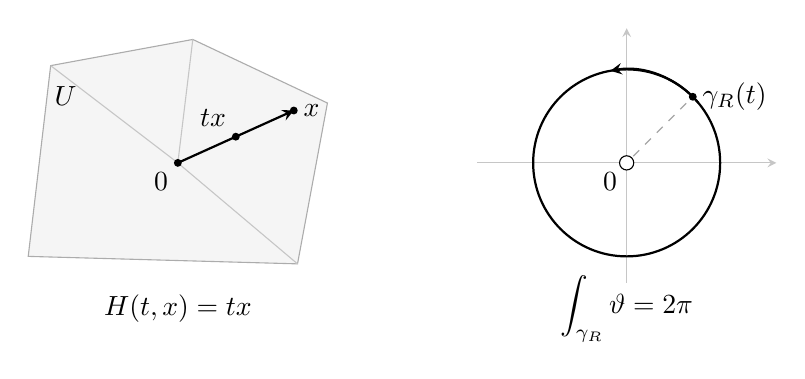
\begin{tikzpicture}[>=stealth,scale=0.95]
		\begin{scope}
			\filldraw[fill=gray!8,draw=gray!65] (-2,-1.25)--(-1.7,1.3)--(0.2,1.65)--(2,0.8)--(1.6,-1.35)--cycle;
			\node at (-1.5,0.9) {\(U\)};
			\draw[gray!45] (0,0)--(-1.7,1.3);
			\draw[gray!45] (0,0)--(0.2,1.65);
			\draw[gray!45] (0,0)--(1.6,-1.35);
			\draw[thick,->] (0,0)--(1.55,0.7);
			\fill (0,0) circle (1.5pt) node[below left] {\(0\)};
			\fill (0.775,0.35) circle (1.5pt) node[above left] {\(tx\)};
			\fill (1.55,0.7) circle (1.5pt) node[right] {\(x\)};
			\node at (0,-1.95) {\(H(t,x)=tx\)};
		\end{scope}
		\begin{scope}[xshift=6cm]
			\draw[gray!45,->] (-2,0)--(2,0);
			\draw[gray!45,->] (0,-1.6)--(0,1.8);
			\draw[thick] (0,0) circle (1.25);
			\draw[thick,->] (40:1.25) arc (40:100:1.25);
			\draw[dashed,gray!70] (0.09,0.09)--(45:1.25);
			\filldraw[fill=white,draw=black] (0,0) circle (2.7pt);
			\node[below left] at (0,0) {\(0\)};
			\fill (45:1.25) circle (1.5pt);
			\node[right] at (45:1.25) {\(\gamma_R(t)\)};
			\node at (0,-1.95) {\(\displaystyle\int_{\gamma_R}\vartheta=2\pi\)};
		\end{scope}
	\end{tikzpicture}
	\caption{左图中，从 \(0\) 到 \(x\) 的径向路径始终留在星形区域内，因此可以沿这一族路径构造原形式。右图的原点被删去，径向收缩不能到达原点；角形式沿圆周的非零周期进一步证明它没有整体原函数。}
	\label{g1:fig:radial-and-period}
\end{figure}


\cref{g1:fig:radial-and-period}把两种构造放在一起：星形区域中径向同伦始终留在定义域内，而穿孔平面中不能把终点设为被删除的原点。穿孔平面上的非恰当性由上面的周期计算证明，不能仅凭一个选定的径向构造失效便作判断。

\ProseParagraphBreak

将角形式限制到单位圆周也得到一个反例。以下取 \(S^1=\{(x,y):x^2+y^2=1\}\)，令 \(j:S^1\hookrightarrow P\) 为包含映射，并记
\[
	\sigma=j^*\vartheta,\qquad
	q:\mathbb R\longrightarrow S^1,\quad q(t)=(\cos t,\sin t).
\]
于是 \(q^*\sigma=\mathrm{d}t\)，沿正向一周的周期为 \(2\pi\)，故 \(\sigma\) 在圆周上不恰当。圆周上的每个一形式都闭，因为二次形式空间为零；所以在一维流形上，闭性本身也不能消除绕圈后的整体障碍。

\begin{proposition}[圆周上的周期判据]
	\label{g1:prop:circle-exactness-period}
	设 \(\lambda\) 为单位圆周 \(S^1\) 上的光滑一形式，写
	\[
		q^*\lambda=a(t)\,\mathrm{d}t,\qquad
		\mathcal P(\lambda)=\int_0^{2\pi}a(t)\,\mathrm{d}t.
	\]
	则 \(a\) 是光滑的 \(2\pi\) 周期函数，且 \(\lambda\) 恰当当且仅当 \(\mathcal P(\lambda)=0\)。更一般地，每个这样的形式都可写成
	\[
		\lambda=c\sigma+\mathrm{d}u,\qquad
		c=\frac{\mathcal P(\lambda)}{2\pi},
	\]
	其中 \(c\) 唯一，光滑函数 \(u:S^1\to\mathbb R\) 在相差常数的意义下唯一。
\end{proposition}
\begin{proof}
	由于 \(q(t+2\pi)=q(t)\) 且 \(q'(t+2\pi)=q'(t)\)，系数 \(a(t)=\lambda_{q(t)}(q'(t))\) 光滑并具有所述周期。若 \(\lambda=\mathrm{d}u\)，沿 \(q|_{[0,2\pi]}\) 使用\cref{g1:lem:exact-path-period}，得到 \(\mathcal P(\lambda)=0\)。

	反过来，设周期为零，令
	\[
		A(t)=\int_0^t a(s)\,\mathrm{d}s.
	\]
	周期性给出 \(A(t+2\pi)-A(t)=\mathcal P(\lambda)=0\)，所以 \(A\) 也为 \(2\pi\) 周期函数。于是可以定义 \(u(q(t))=A(t)\)：两个实数给出同一圆周点时相差 \(2\pi\) 的整数倍，故这个值与代表无关。

	还须检查下降后的函数光滑。\(q'(t)\) 从不为零，由\cref{g1:thm:inverse-function}，\(q\) 在每点附近到一个圆周小弧是微分同胚；在这个小弧上，\(u\) 就是光滑函数 \(A\) 与光滑局部角坐标的复合。因此 \(u\) 光滑。又有
	\[
		q^*(\mathrm{d}u)=\mathrm{d}(u\circ q)=\mathrm{d}A
		=a(t)\,\mathrm{d}t=q^*\lambda.
	\]
	\(q\) 满射且局部微分同胚，每个圆周切向量都能在某个实数点由其微分得到，所以拉回相等蕴含 \(\mathrm{d}u=\lambda\)。

	对一般 \(\lambda\)，取 \(c=\mathcal P(\lambda)/(2\pi)\)，则 \(\lambda-c\sigma\) 的周期为零，刚才的结论给出所需 \(u\)。若存在另一种分解，取周期便知常系数同为 \(c\)；随后两个原函数之差的微分为零。圆周连通，局部常值结论使它们只差常数。
\end{proof}

例如 \(\sigma\) 没有整体原函数，但 \(x\sigma\) 有：在角参数中，它的拉回为 \(\cos t\,\mathrm{d}t=\mathrm{d}(\sin t)\)，所以 \(x\sigma=\mathrm{d}(y|_{S^1})\)。而 \((1+x)\sigma\) 的周期仍为 \(2\pi\)，不恰当。这里决定能否取整体原函数的是一周累积的周期，而不是形式在某个局部坐标中的系数是否为零。
% 纲要条目排为编号小节标题，并进入目录与书签；说明段仍保留于纲要注释中。
